\section{Class Diagrams}

%	Sottolineare il target di tecnologie per cui è effettuata la progettazione. Queste non verranno citate all'interno del capitolo
%	di Progetto ma, il seguente capitolo di Realizzazione, introducendo banalmente le tecnologie utilizzate, dovrà poter
%	calzare perfettamente e dovrà facilmente potersi riallacciare a quanto detto in questo capitolo.

%	In questa sezione si ripercorrono gli stessi argomenti della parte di analisi, in parallelo, ma focalizzandosi sulle scelte di
%	progetto. Queste dovranno essere motivate e lo scopo di questa porzione di testo è di definire le varie parti e la loro 
%	collaborazione GLOBALE (API + persistenza). Il livello di dettaglio non sarà massimo in quanto nelle successive sezioni 
%	si entrerà nello specifico.
%
%	{Diagrammi} Class diagrams UML o analoghi più efficaci per il comportamento dinamico
%	{Immagini}

\section{API}

%	{Analisi prettamente tecnologica}
%	
%	Qui, sulla base di quanto detto nella sezione di analisi, si inizia a mettere insieme le varie parti per descrivere più
%	nel dettaglio l'API dal punto di vista progettuale. Già nella prima parte di analisi è stato introdotto a grandi linee il funzionamento.
%	
%	Il focus è sulle scelte progettuali. Evidenziare dunque i punti di forza e le scelte a livello di pattern.

	Nei successivi paragrafi si spiegherà più nel dettaglio ogni parte attiva all'interno del progetto di queste API, illustrandone e motivandone tutte le scelte progettuali rilevanti.
	Come già deducibile dalla precedente sezione, le API consistono fondamentalmente di due interfacce, \textit{stabili}, \textit{comuni} e \textit{unificate}, che forniscono \textit{Protected Variation} rispetto a rivisitazioni e ottimizzazioni. Pertanto sono state per fornire all'utilizzatore un punto di contatto singolo, una \textit{Facade}, con le librerie.
	
	
	\subsection{Interfaccia ADS}
	
	%	MODELLO FUNZIONALE, motivare la necessità
	%
	%	Sezione in cui si motiva pattern per interfaccia e si evidenzia collegamento funzionale con casi d'uso e requisiti, in termini solo di funzionalità offerte
	
		L'interfaccia dell'ADS, è stata resa parametrica rispetto a tre valori:
		
		\begin{itemize}
			\item \textbf{H}: il tipo dei vari \textit{hash} presenti all'interno dei nodi della struttura.
			\item \textbf{K}: il tipo delle \textit{chiavi} dei nodi.
			\item \textbf{V}: il tipo dei valori presenti nello \textit{storage}. 
		\end{itemize}
	
		Questa scelta rende l'interfaccia applicabile parametricamente rispetto alla scelta dei suddetti tipi, caratteristica utile per garantire flessibilità. 

		Le operazioni fornite dall'ADS, sulla base di requisiti e casi d'uso già discussi in fase di analisi, sono:
		\begin{itemize}
			\item \textbf{\textit{getWithProof(k)}}: restituisce il valore $ v $ associato alla chiave $ k $, assieme alla \textit{Proof} per quella chiave. Questa operazione è necessaria per permettere di ottenere la Proof relativa ad una specifica coppia chiave-valore $ (k,v) $.
			\item\textbf{ \textit{getProof(keys)}}: restituisce la Proof relativa alle chiavi contenute nella lista \textit{keys}. Estende le possibilità di \textit{getWithProof(k)}, restituendo in un solo round una Proof cumulativa per un'insieme di chiavi $ keys $, valida e utilizzabile per tutte le stesse. 
			\item \textbf{\textit{getValue(key)}}: data una chiave $ k $, restituisce il valore $ v $ associato ad essa. Questa operazione permette dunque le operazioni di lettura, \textit{read(k)}, richieste dai casi d'uso.
			\item \textbf{\textit{add(k, v)}}: crea un \textit{delta} rispetto alla struttura corrente, il quale viene memorizzato. Il delta riguarda l'aggiunta o la modifica degli elementi relativi alla chiave $ k $. L'operazione \underline{non} modifica la struttura corrente.
			\item \textbf{\textit{del(k)}}: crea un \textit{delta} rispetto alla struttura corrente, il quale viene memorizzato. Il delta riguarda la cancellazione degli elementi relativi alla chiave $ k $ L'operazione \underline{non} modifica la struttura corrente.
			\item \textit{applyDeltas()}: compatta tutti i vari delta relativi alla struttura corrente e li applica in ordine, restituendo una nuova ADS, con le modifiche applicate. Questa operazione permette all'ADS di avere la capacità di aggiornarsi rispetto a richieste di update in arrivo dai client.
			\item \textit{rootHash()}: calcola e restituisce il \textit{Root Hash} della struttura corrente. Questa operazione permette di ottenere il \textit{digest} dell'intera struttura, come specificato dai requisiti.
			\item \textit{isEmpty()}: Informa se l'ADS è vuoto o meno.
		\end{itemize}
	
		E' necessario sottolineare riguardo alla prima operazione fornita, che, per \textit{Creator}, sara l'ADS stesso a generare una Proof una o più chiavi, proprio in quanto è l'unica entità a conoscere le informazioni per farlo. A seguito della creazione, essa sarà un entità indipendente, in grado di aggiornarsi in parallelo rispetto agli update. I calcoli e le operazioni poi eseguite sulla Proof, sono indipendenti dall'ADS di partenza.
		
		Di fondamentale importanza è il requisito relativo alla possibilità di utilizzo dell'ADS in ambito concorrente. Deve essere possibile, dunque, poter operare operazioni in parallelo sull'ADS, senza che ci siano conflitti dovuti alla concorrenza. Pertanto è stato deciso di applicare un principio tipico del paradigma di programmazione funzionale, secondo cui i valori non vengono trovati cambiando lo stato dell'ADS, ma costruendo nuovi stati a partire dai precedenti. Per questo motivo le operazioni di scrittura, ovvero quelle che modificherebbero lo stato della struttura, lo fanno in maniera totalmente compatibile con quanto detto. Una spiegazione più dettagliata di come questo sia stato realizzato è posticipata in paragrafi successivi.
		
		La scelta invece di disaccoppiare il momento dell'individuazione della operazioni di aggiunta, modifica o cancellazione, dal momento della loro effettiva applicazione, è da inquadrare in un contesto più ampio di utilizzo della libreria. Intuitivamente, questa funzionalità è fornita per permettere di gestire meglio gli stati in cui si può trovare la struttura stessa: ad esempio uno stato in cui può ricevere e accumulare update, piuttosto che uno stato in cui questi vengono applicati in blocco. Migliore è di conseguenza la gestione delle operazioni di lettura, in quanto per garantirne la consistenza, esse possono essere collocate in istanti temporali diversi, prima o dopo determinati stati della struttura.
		
		L'interfaccia, e dunque la classi che implementeranno quest'ultima, deve implementare a sua volta l'interfaccia \textit{Serializable}, in quanto dovrà avere la caratteristica di essere, appunto, serializzabile. Questo è motivato dal fatto che implementazioni di questa interfaccia saranno inserite all'interno di messaggi che dovranno essere spediti su rete, nell'ambito dell'utilizzo di questa API.
	
	\subsection{Interfaccia Proof}
	
	%	MODELLO FUNZIONALE, motivare la necessità
	%
	%	Sezione in cui si motiva pattern per interfaccia e si evidenzia collegamento funzionale con casi d'uso e requisiti, in termini solo di funzionalità offerte
		
		L'interfaccia della Proof, è stata resa parametrica rispetto a tre valori:
		
		\begin{itemize}
			\item \textbf{H}: il tipo dei vari \textit{hash} presenti all'interno dei nodi della Proof.
			\item \textbf{K}: il tipo delle \textit{chiavi} dei nodi.
			\item \textbf{V}: il tipo dei valori presenti nello \textit{storage}. 
		\end{itemize}
		
		Questa scelta rende l'interfaccia applicabile parametricamente rispetto alla scelta dei suddetti tipi, caratteristica utile per garantire flessibilità. 
		
		Le operazioni fornite dalla Proof, sulla base di requisiti e casi d'uso già discussi in fase di analisi, sono:
		\begin{itemize}
			\item \textbf{\textit{keys: Set<K>}}: insieme contenente tutte le chiavi per cui è valida la Proof.
			\item \textbf{\textit{rootHash(): H}}: restituisce il \textit{Root Hash} della Proof. Questa, assieme alla successiva, sono requisiti funzionali già discussi in fase di analisi.
			\item \textbf{\textit{rootHash(list: List<Pair<K, V>>): Proof<H, K, V>}}: applica gli aggiornamenti specificati nella lista di coppie chiave-valore \textit{list} e successivamente calcola e restituisce il nuovo \textit{Root Hash}.
			\item \textbf{\textit{union(proof: Proof<H, K, V>): Proof<H, K, V>}}: effettua il \textit{merge} di due Proof relative allo stesso istante temporale della stessa struttura da cui sono state generate. Restituisce una nuova proof, cumulativa rispetto a quelle di partenza.
		\end{itemize}
		
		Di fondamentale importanza è il requisito relativo alla possibilità di utilizzo della Proof in ambito concorrente. Deve essere possibile, dunque, poter operare operazioni in parallelo sulla Proof, senza che ci siano conflitti dovuti alla concorrenza. Pertanto è stato deciso di applicare un principio tipico del paradigma di programmazione funzionale, secondo cui i valori non vengono trovati cambiando lo stato della Proof stessa, ma costruendo nuovi stati a partire dai precedenti. Per questo motivo le operazioni di scrittura, ovvero quelle che modificherebbero lo stato della struttura, lo fanno in maniera totalmente compatibile con quanto detto. Una spiegazione più dettagliata di come questo sia stato realizzato è posticipata in paragrafi successivi.
		
		L'interfaccia, e dunque la classi che implementeranno quest'ultima, deve implementare a sua voltal'interfaccia \textit{Serializable}, in quanto dovrà avere la caratteristica di essere, appunto, serializzabile. Questo è motivato dal fatto che implementazioni di questa interfaccia saranno inserite all'interno di messaggi che dovranno essere spediti su rete, nell'ambito dell'utilizzo di questa API.
	
	\subsection{Nodo e schema hashing}
	
	%	Parlare dell'elemento alla base di implementazioni realizzate di ADS e Proof.
	%
	%	Breve sezione che riprende l'argomento dell'hashing e che lo analizza concentrandosi sulle scelte progettuali. Si parla anche della parametrizzazione rispetto
	%	alle varie funzioni di hashing e si parla di HashUtils con relativo pattern Singleton
	
	L'elemento base costituente sia della Skip List Autenticata sia della Skip List Proof, è il \textit{nodo}. Esso, oltre ad essere a conoscenza dei suoi nodi adiacenti, nelle quattro direzioni, \textit{next}, \textit{prev},  \textit{up} e \textit{down}, è formato da tre campi interni:
	\begin{itemize}
		\item \textbf{Key}: Un attributo chiave necessario per la struttura in cui è collocato a mantenere l'ordinamento. Il tipo $ K $ della chiave \underline{deve} dunque necessariamente implementare l'interfaccia \textit{Comparable<K>}.
		\item \textbf{First Hash}: Un campo che contiene l'hash relativo al nodo immediatamente inferiore , \textit{down} ,o l'hash del valore dello storage relativo a questo nodo.
		\item \textbf{Second Hash}: Un campo che contiene l'hash relativo al nodo successivo,  \textit{next}, se quest'ultimo è presente.
	\end{itemize}

	La scelta di tripartire all'interno del nodo le sezioni sopra menzionate, è stata presa sia per poter rispettare nella maniera più comoda e flessibile lo schema di hashing già discusso in fase di analisi, e sia per ridurre la quantità di operazioni per il refresh di tutta la struttura, a seguito di operazioni di update. Infatti a seguito di una operazione di inserimento, modifica o cancellazione, sarà necessario aggiornare solamente i campi strettamente interessati.
	
	Il campo \textit{down}, si precisa, che può essere sia una nodo, nella maggior parte dei casi, ma anche il valore vero e proprio, presente nello storage classico, legato a questo nodo. Sarà dunque solo ed esclusivamente questo nodo a conoscere questo valore e a memorizzare il suo hash nel campo \textit{first Hash}.
	
	La classe che implementa il nodo, deve implementare l'interfaccia \textit{Serializable}, in quanto dovrà avere la caratteristica di essere, appunto, serializzabile. Questo è motivato dall'inserimento di oggetti di questo tipo all'interno di messaggi che dovranno essere spediti su rete, nell'ambito dell'utilizzo di questa API.
	
	Lo schema di hashing presente all'interno della struttura, rispecchia quello già presentato in fase di analisi, e si adatta perfettamente alla separazione dei valori di hash attuata all'interno del nodo. Infatti da un lato il campo \textit{first Hash}, memorizzerà sempre l'hash relativo al campo \textit{down} del nodo, sia esso un nodo o un valore vero e proprio, di tipo qualsiasi. Dall'altro lato il campo \textit{second Hash} memorizzerà, solo se presente, l'hash relativo al campo \textit{next} del nodo corrente. 
	E' stato ritenuto conveniente eliminare, per i nodi sulla \textit{base list}, il fatto che il campo \textit{second Hash}, nel caso in cui il nodo \textit{next} sia un nodo \textit{tower}, dovesse memorizzare l'hash relativo al valore sottostante il nodo \textit{next}. Questo permette di garantire l'esecuzione di tutte le operazione che comportino un refresh degli hash della struttura, in un tempo che sia con alta probabilità, $\mathcal{O}(log{}n)$.
	Inoltre, la proprietà di non-commutatività degli hash, si manifesta nel fatto che, per costruzione, se fosse invertito il valore presente nel campo \textit{first Hash}, con quello presente nel campo \textit{second Hash}, il cambiamento si ripercuoterebbe su tutti gli hash seguenti, fino ad arrivare alla modifica del root Hash dell'intera struttura. Pertanto è fondamentale l'ordine e la posizione reciproca dei vari nodi.
	
	Per quanto riguarda più specificatamente le funzioni crittografiche di hash, si è deciso di delegare il compito di calcolo di hash, singoli o concatenati, ad un \textit{Singleton}, visibile a tutte le classi dell'API. Questa scelta ha permesso di rendere l'intera realizzazione totalmente flessibile e parametrica rispetto alla particolare funzione di hash che si volesse adottare.
	
	\begin{figure}
		\centering
		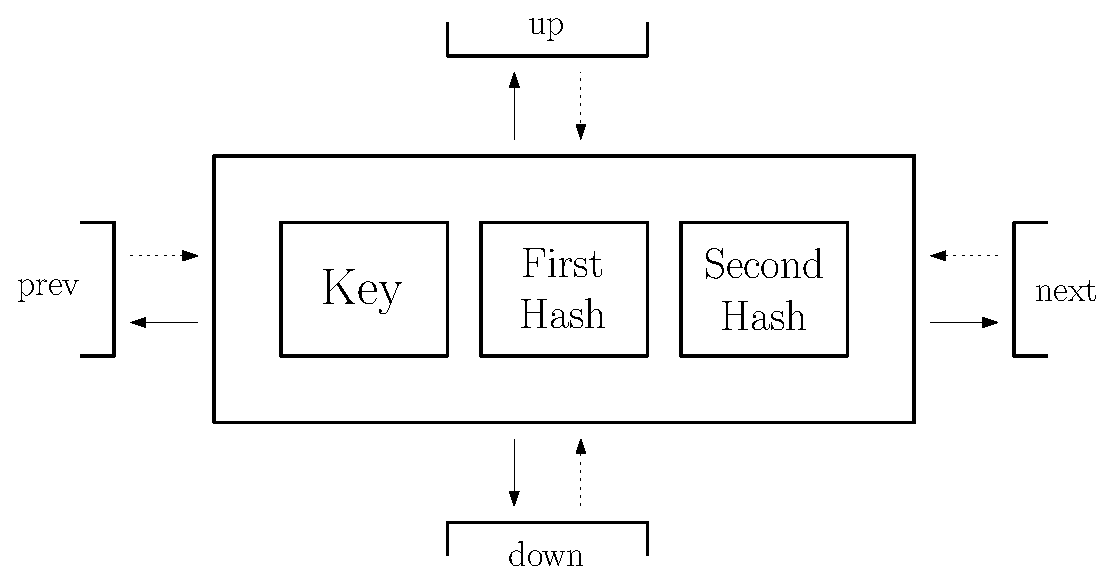
\includegraphics[scale=0.6]{figure/nodo.eps}
		\caption{Esempio di un nodo.}\label{fig:1}
	\end{figure}
		
	\subsection{Skip List Autenticata}
	
	%	MODELLO FUNZIONALE, motivare la realizzazione
	%	
	% 	Fatte tutte le opportune premesse descritte e motivate (APS style), si passa ora alla descrizione della struttura principale
	
	Prima di addentrarsi dettagliatamente sulla parte progettuale e algoritmica della struttura dati autenticata, è necessario fare delle considerazioni di carattere generale, conseguenza di quanto detto in fase di analisi.
	Prima di tutto si sottolinea l'inutilità, in questo studio progettuale, della colonna di nodi sentinella di tipo $ +\infy $, la cui presenza comporterebbe solo un inutile spreco di memoria. I nodi sentinella di tipo $ -\infy $, d'altro canto, servono sia per poter avere una colonna che sia concettualmente antecedente a tutte le altre colonne presenti nella struttura e sia di supporto all'applicazione dello schema di hashing.
	Secondariamente si è ritenuto superfluo, e puramente formale, il mantenimento di un livello superiore a tutti gli altri livelli, contenente soltanto agli estremi i nodi sentinella. Questo aggiungerebbe solamente una passo in più agli algoritmi di esecuzione delle operazioni. Nel contesto più ampio di una successiva applicazione di memorizzazione in persistenza della struttura, il mantenimento di questo livello superiore  complicherebbe soltanto la conversione da formato ad oggetti al formato della base di dati.
	
	La ricerca in tempo logaritmico, cosi come le operazioni di inserimento, cancellazione o modifica, sono permesse dalle chiavi dei nodi, che dunque saranno ordinate: $ k_{-\infty} < k_{1} < k_{2} < \dots < k_{n} < k_{+\infty} $.
	
	\subsection{Skip List Proof}
	
	%	MODELLO FUNZIONALE, motivare la realizzazione
	%	
	%	Fatte tutte le opportune premesse descritte e motivate (APS style), si passa ora alla descrizione della struttura proof














	
\section{Persistenza}

%	Introduzione al discorso sulla persistenza, riallacciandosi a ciò che è stato detto nella parte di analisi.
%	
%	VISTO CHE NON SARA' PRESENTE UNA PARTE DI REALIZZAZIONE PER LA PARTE DI PERSISTENZA, E DUNQUE
%	NON SARA' POSSIBILE PARLARE DELLA TECNOLOGIE UTILIZZATE, CERCARE DI SOTTOLINEARLO INDIRETTAMENTE QUI,
%	PUR SEMPRE APPUNTO NON CITANDO ESATTAMENTE LE TECNOLOGIE CHE SI E' PENSATO DI APPLICARE.
		
	\subsection{Studi teorici}
		
%		Qui viene affrontato il problema dal punto di vista teorico, con particolare attenzione a sottolineare i problemi teorici derivati dallo studio 
%		teorico operato per quanto riguarda la persistenza di una struttura dati su base di dati NoSQL. Qui darei un accento più teorico, mentre le 
%		scelte progettuali che ne possono derivare, le descriverei nelle successive sezioni.
		
	\subsection{Progettazione}
	
%	Questa è la sezione in cui si parla di tutto il progetto legato alla persistenza, e di come questo si lega al tutto.
%	E' importante qui accennare tutti gli attori e la loro interazione globale. Il focus è sulle scelte progettuali, e sui
%	pattern applicati, ma saranno descritti al massimo livello di dettaglio solo nelle sottosezioni successive.
		
	\subsection{Translator}
	
%		Entro nel dettaglio del Translator, descrivendo compiti e giustificandolo tramite pattern
		
	\subsection{Connector}
	
%		Entro nel dettaglio del Connector, descrivendo compiti e giustificandolo tramite pattern
	
	\subsection{CassandraService}
	
%		Entro nel dettaglio del Service, descrivendo compiti e giustificandolo tramite pattern.
%		Enfasi su come questa parte sia un centro-stella per le altre parti progettuali
		
	\subsection{Comportamento asincrono}
	
%		In base a quanto detto, sottolineare le decisioni progettuali e di come queste possano essere ottimizzate con
%		comportamento asincrono. Sottolineare bene che uno degli obiettivi è stato quello di minimizzare i round di 
%		query con Cassandra, e che questo è reso possibile da coroutine tipiche di linguaggi di programmazione OO moderni.
			
	\subsection{Caching}
	
%		In questa parte si analizza il problema di caching con relativi problemi di "always-on". Descrivere compiti e giustificazioni
%		tramite pattern e future proofing. Giustificare anceh in funzione del contesto piu generale delle dimensioni dell'ADS (fare calcolo su stime)